\subsubsection{Latency \& Throughput}

Charts on Figures \ref{fig:persistent_transport_latency}, \ref{fig:ephemeral_transport_latency}, \ref{fig:persistent_transport_throughput}, and \ref{fig:ephemeral_transport_throughput} represent the \gls{p90} of Latency and Throughput of all 10000 requests made by the persistent and ephemeral clients during the experiments.

\subsubsection*{Scenarios Pattern}

Throughout experiments it is possible to observe a pattern. Local scenarios usually had better performance when compared to Single-\gls{az} and Multi-\gls{az} scenarios. This happens because, by using localhost, the traffic never leaves the host machine, it bypasses any local network interface hardware, being executed exclusively via software \cite{rfc4291}.

All other scenarios are limited by the networking capabilities of the AWS' EC2 instance, which is around 12.5Gb/s \cite{m6i_xlarge_aws_ec2}. Thus, Local-AZ and Multi-AZ scenarios can only reach a theoretical maximum of 12.5Gb/s of throughput, while Local scenario is not affected by such limits.

Additionally, the Single-\gls{az} scenarios were better than Multi-\gls{az} scenarios due to the overhead from sending the datagram to another data center. Even though remaining in the same region, it results in a higher latency.

\subsubsection*{\gls{udp} Unreliability}

\gls{udp} Multi-\gls{az} and Single-\gls{az} experiments only succeeded on the first two iterations of each run when the data transferred was 2KiB and 8KiB. This was expected since pure \gls{udp} does not have any reliability and is expected to lose user datagrams along the way. As was stated before, no additional logic was added to \gls{udp} since this would interfere with the results because it would alter \gls{udp} natural behaviour.

\subsubsection*{TCP is more optimized than UDP}

Local \gls{tcp} experiment was by far the most efficient, with almost zero latency when connection was persistent, reaching approximately 19Gb/s of speed (Figure \ref{fig:persistent_transport_latency}) when transferring 512KiB of data per request. It outperformed \gls{udp}, that even though is considered faster due to its unreliability and connectionless characteristics, it only reached 2.8Gb/s in the same scenario. 

\gls{tcp} is considered a stream oriented protocol, it receives a stream of bytes from the application-layer and it's his responsibility to divide it into segments before passing it on. \gls{udp} on the other hand, is considered a message oriented protocol, it defers the burden of dividing the streams of data into messages to the application-layer. While TCP's data division is implemented in the kernel, UDP's depends on the application. Thus, TCP is able to have a higher througput than UDP.

\subsubsection*{Connection Establishment Impact}

Ephemeral clients demonstrated that establishing connections can have a significant impact on \gls{tcp}’s performance. Local \gls{tcp} latency went from 0.19ms to 1.79ms and throughput from 19Gb/s to 2.2Gb/s (Figures \ref{fig:persistent_transport_latency} and \ref{fig:ephemeral_transport_latency}). Both results are still better than other \gls{tcp} and all \gls{tcp}+\gls{tls}’ experiments, but brings them to a similar level.

\subsubsection*{\gls{tls} Overhead}

As expected, \gls{tls} encryption adds a slight overhead on \gls{tcp} during persistent clients experiments (Figures \ref{fig:persistent_transport_latency} and \ref{fig:persistent_transport_throughput}), as it needs to perform a \gls{tls} handshake, consequently adding couple of extra \gls{rtt}s to be able to establish a connection. 

This difference is amplified during ephemeral client experiments (Figures \ref{fig:ephemeral_transport_latency} and \ref{fig:ephemeral_transport_throughput}) due to having to perform a \gls{tls} handshake before every request.

\subsubsection*{QUIC \& \gls{udp}}

Though \gls{udp} have a higher throughput than QUIC, they share a common pattern. This can be better observed during Local experiments with persistent clients (Figure \ref{fig:persistent_transport_throughput}). This similarity exists since QUIC uses \gls{udp} as its underlying transport mechanism, therefore it shares the same limitations as \gls{udp}.

\subsubsection*{QUIC's Handshake Efficiency}

Although QUIC did not perform nearly as well as TCP+TLS, it managed to be less impacted by ephemeral clients.

During the Multi-AZ scenario, while TCP+TLS’ throughput went from 3160 Mb/s with persistent clients to 668 Mb/s with ephemeral clients, equivalent to a decrease of 79\%, QUIC’s throughput went from 487 Mb/s to 231 Mb/s, equivalent to a decrease of 52\% (Figures \ref{fig:persistent_transport_throughput} and \ref{fig:ephemeral_transport_throughput}). This demonstrates the impact of QUIC’s handshake since it only needs 1-\gls{rtt} with unknown servers, while TCP+TLS’ handshake requires, in general, 3-\gls{rtt}s.

\subsubsection*{QUIC's Bad Performance}

QUIC’s experiments were the worst, with latency and throughput almost 6 times worse than \gls{tcp}+\gls{tls}’ during Multi-\gls{az} with persistent client experiment (Figures \ref{fig:persistent_transport_latency} and \ref{fig:persistent_transport_throughput}).

As this is a cloud environment, packet loss rate is pretty low, resulting in a reliable network. QUIC’s main purpose is to improve performance of devices operating in an unreliable network, such as wireless and mobile networks. Thus, QUIC’s benefits can only be seen when it’s used in an environment with a high rate of packet loss.

One of the main reasons why QUIC is less efficient than TCP+TLS, it’s possibly because TCP’s implementation is more efficient than UDP’s. As QUIC has UDP as its bottleneck and UDP is worse than TCP on a reliable network, QUIC can only be as efficient as UDP. Consequently, it will not be able to surpass TCP’s performance with UDP’s current limitations.

QUIC’s results show it's not meant to be used on distributed systems. These applications are usually contained in environments with reliable networks, meaning that \gls{tcp}+\gls{tls} will, for the time being, be a better fit.

\clearpage

\begin{figure}[h!]
    \centering
    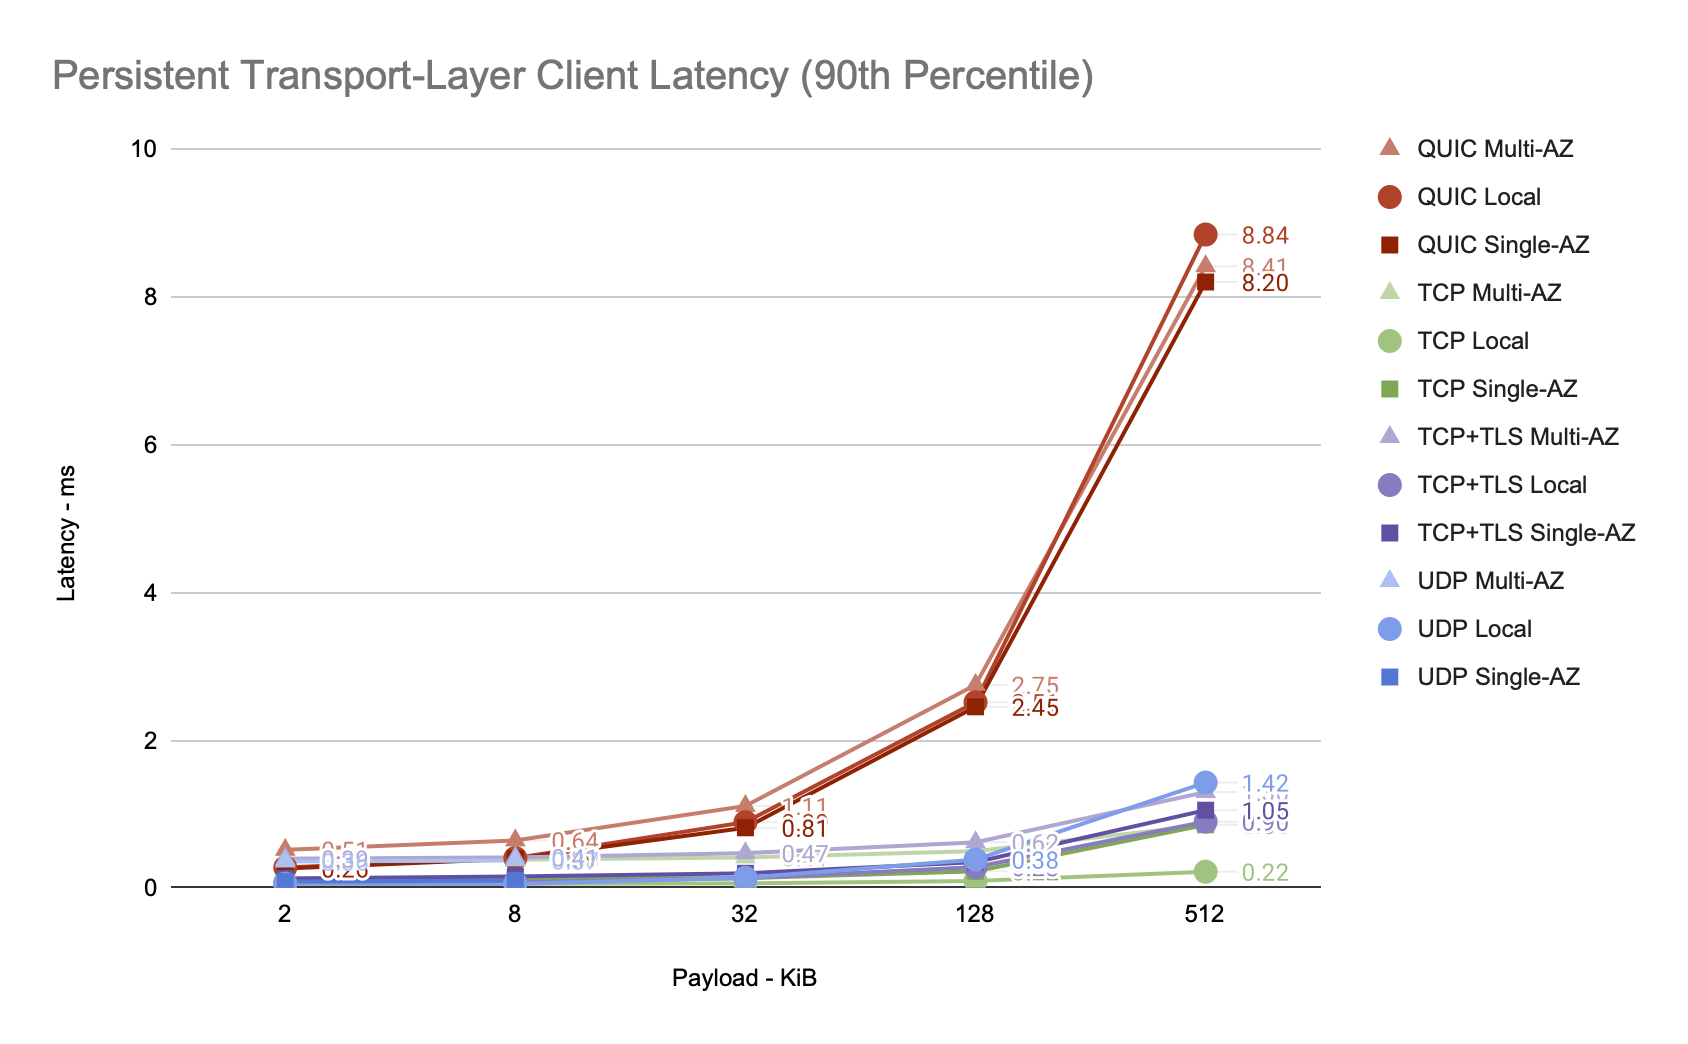
\includegraphics[width=\linewidth]{figures/charts/Persistent Transport-Layer Client Latency (90th Percentile).png}
    \caption{Persistent Transport-Layer Client Latency (90th Percentile)}
    \label{fig:persistent_transport_latency}
\end{figure}

\begin{figure}[h!]
    \centering
    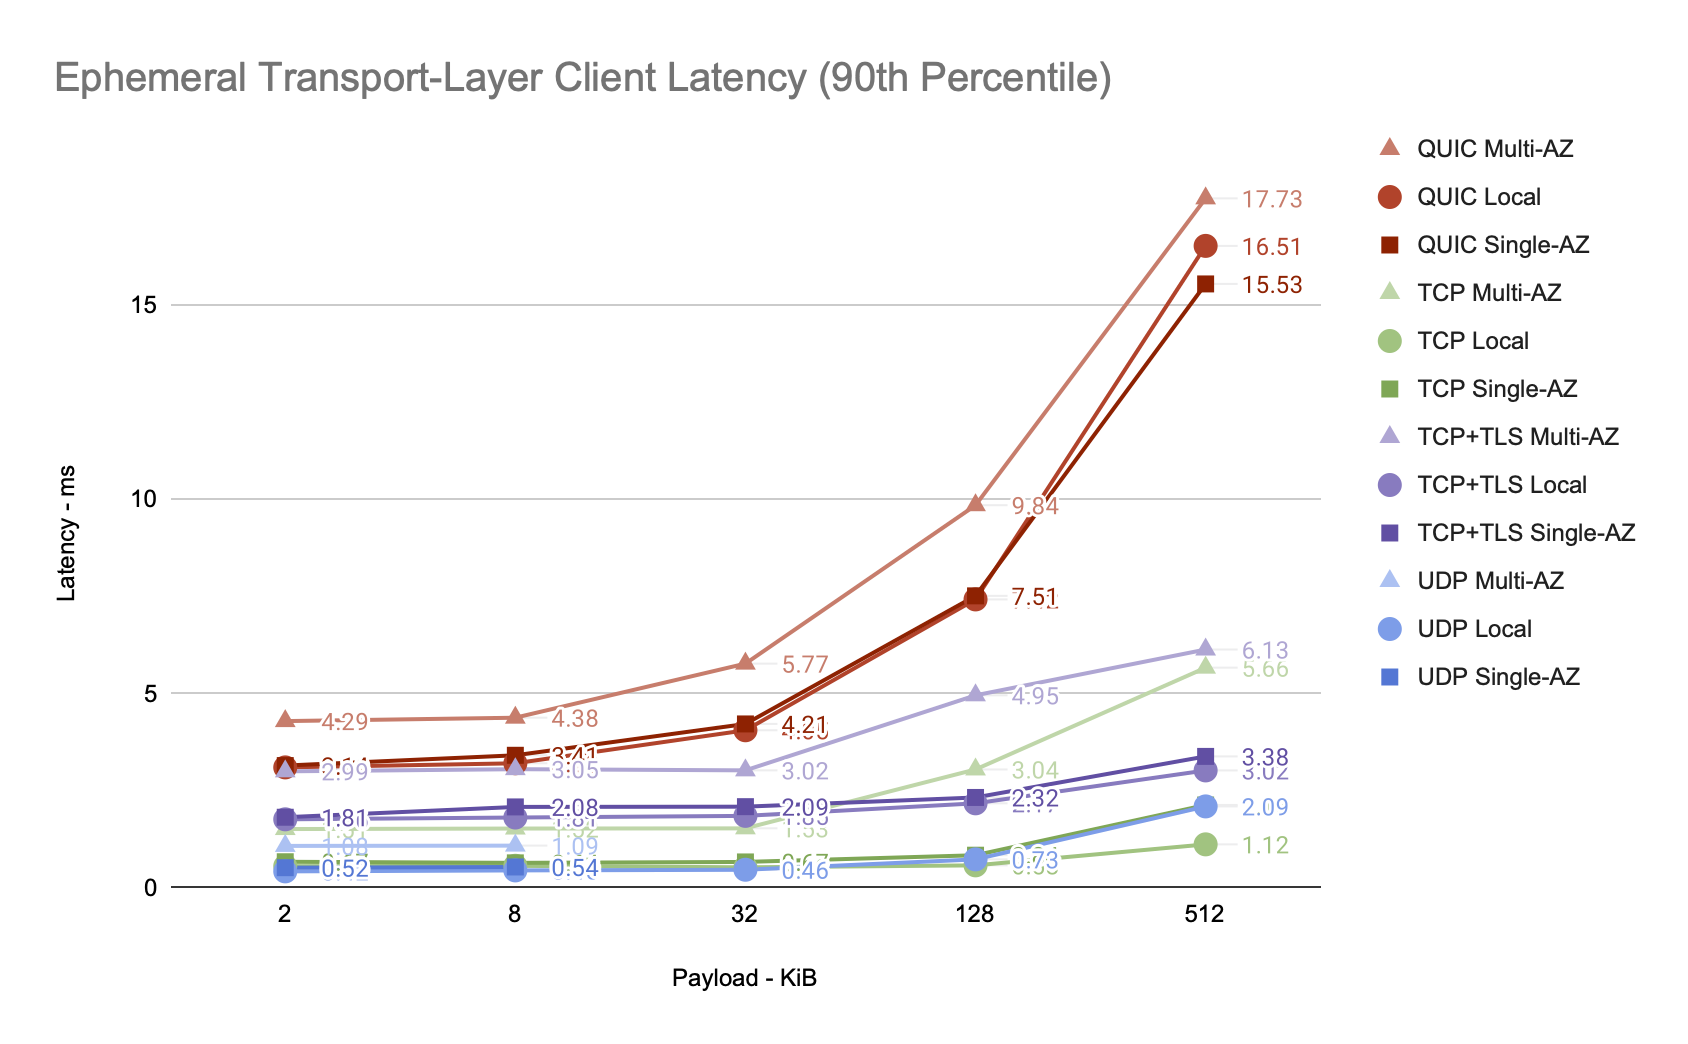
\includegraphics[width=\linewidth]{figures/charts/Ephemeral Transport-Layer Client Latency (90th Percentile).png}
    \caption{Ephemeral Transport-Layer Client Latency (90th Percentile)}
    \label{fig:ephemeral_transport_latency}
\end{figure}

\clearpage

\begin{figure}[h!]
    \centering
    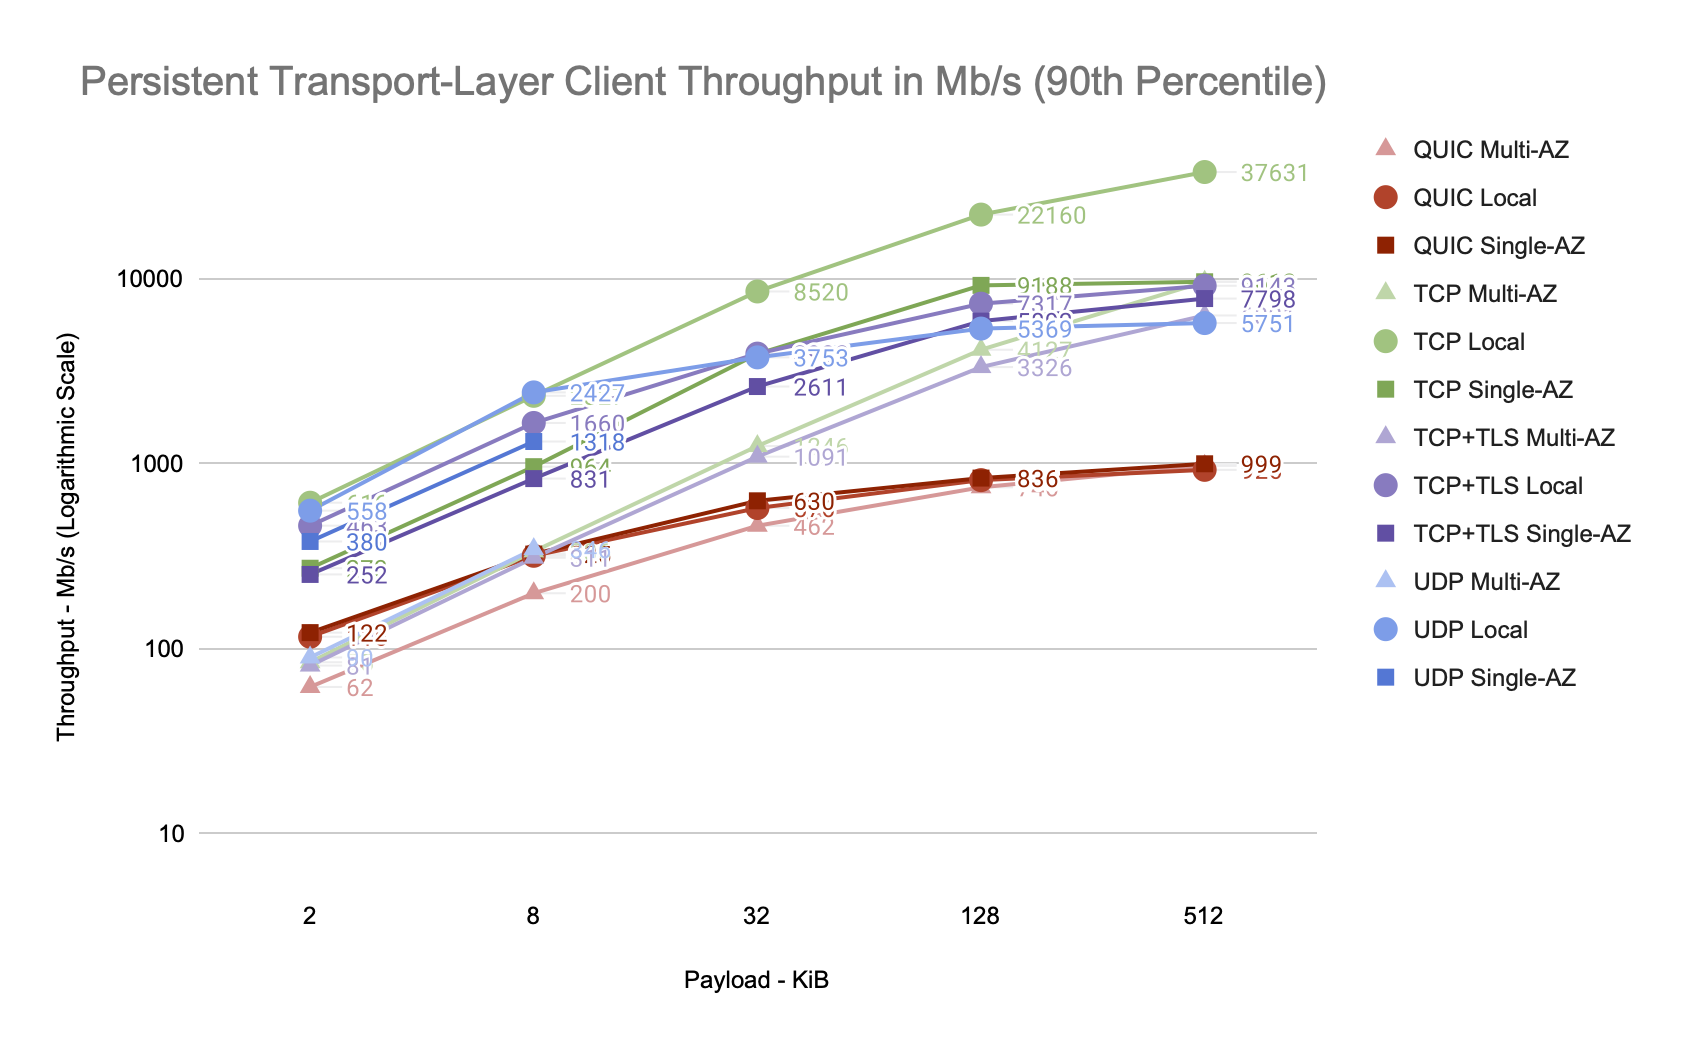
\includegraphics[width=\linewidth]{figures/charts/Persistent Transport-Layer Client Throughput in Mb_s (90th Percentile).png}
    \caption{Persistent Transport-Layer Client Throughput in Mb/s (90th Percentile)}
    \label{fig:persistent_transport_throughput}
\end{figure}

\begin{figure}[h!]
    \centering
    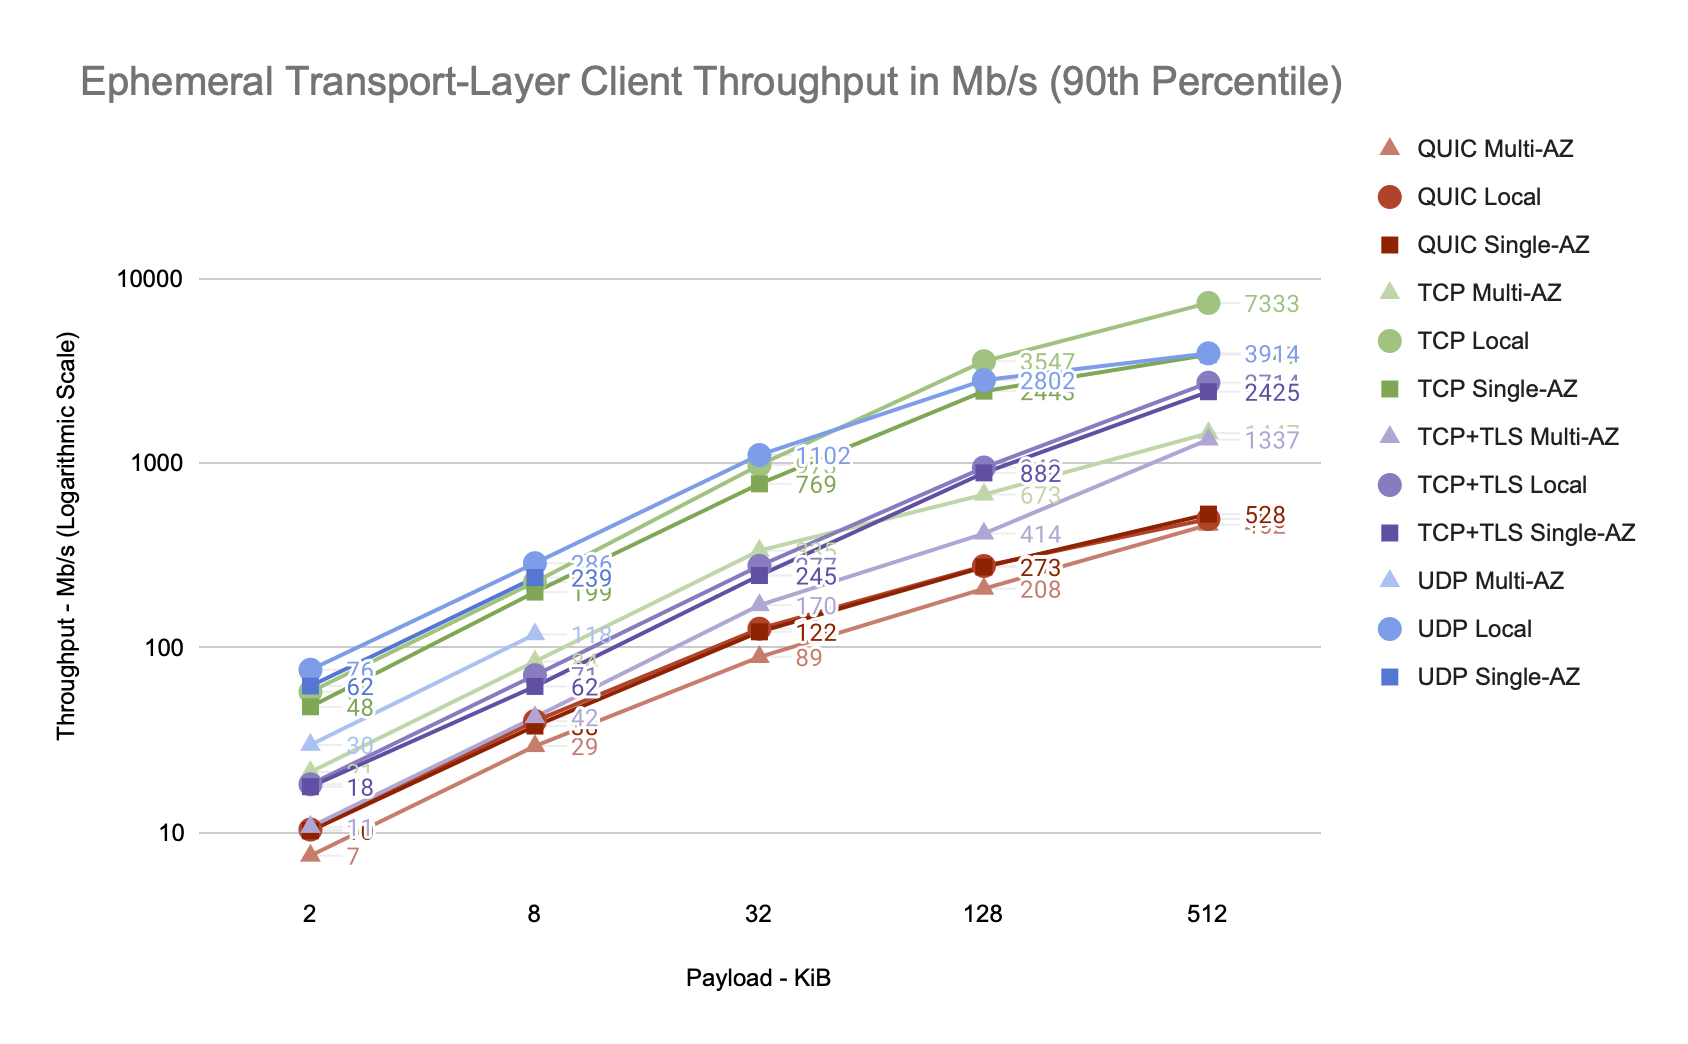
\includegraphics[width=\linewidth]{figures/charts/Ephemeral Transport-Layer Client Throughput in Mb_s (90th Percentile).png}
    \caption{Ephemeral Transport-Layer Client Throughput in Mb/s (90th Percentile)}
    \label{fig:ephemeral_transport_throughput}
\end{figure}

\clearpage
